\section{Countermeasures}
\subsection{ASLR and PIE}
    \frame{
        \frametitle{ASLR and PIE}
        \begin{itemize}
            \item \aslr
            \item \pie
            \item take effect at load and link time during program startup
            \item in the \pax\ implementation, addresses of segments are randomized:
                  \begin{itemize}
                      \item \pgm{.text}-segment of the binary (\lto\ executable code)
                      \item dynamically linked libraries
                      \item the stack
                      \item the heap
                  \end{itemize}
            \item libraries in themselves are not randomized \\
                  \lto\ randomization can be overcome by brute-force attacks and/or through information leakage
        \end{itemize}
    }




\subsection{Stack canaries and shadow stacks}
    \frame{
        \frametitle{Stack canaries -- Explanation}
        \begin{itemize}
            \item canary: word between local variables of a function and the return address
            \item function epilogue: canary word is verified by comparison to a stored value
            \item word has changed \lto\ the canary is dead \Frowny\ \lto\ program is terminated
            \item Example: \sguard
        \end{itemize}
    }

    \frame{
        \frametitle{Stack canaries -- Diagram}
        \begin{center}
            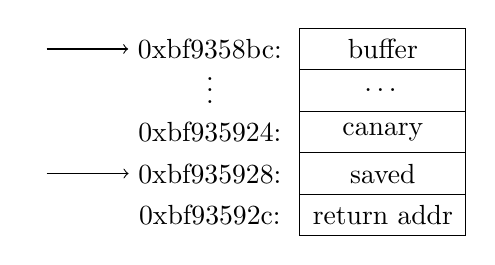
\begin{tikzpicture}
                \tikzset{x=2.5em, y=1.5em}
                \tikzstyle{mem}=[rectangle, draw, minimum width=6em, minimum height=1.5em]

                \draw (0.0, 4.0)    node        (esp)   {\esp};
                \draw (0.0, 1.0)    node        (ebp)   {\ebp};

                \draw (2.5, 4.0)    node        (a4)    {0xbf9358bc:};
                \draw (2.5, 3.2)    node        (a3)    {$\vdots$};
                \draw (2.5, 2.0)    node        (a2)    {0xbf935924:};
                \draw (2.5, 1.0)    node        (a1)    {0xbf935928:};
                \draw (2.5, 0.0)    node        (a0)    {0xbf93592c:};

                \draw (5.0, 4.0)    node[mem]   (buf0)  {buffer};
                \draw (5.0, 3.0)    node[mem]   (buf1)  {\dots};
                \draw (5.0, 2.0)    node[mem]   (sebp)  {canary};
                \draw (5.0, 1.0)    node[mem]   (sebp)  {saved \ebp};
                \draw (5.0, 0.0)    node[mem]   (raddr) {return addr};

                \draw [->]          (esp) -- (a4);
                \draw [->]          (ebp) -- (a1);
            \end{tikzpicture}
        \end{center}
    }

    \frame{
        \frametitle{Shadow stacks}
        \begin{itemize}
            \item \truss: maintains \shadow, which stores return addresses
            \item function prologues: modified to store correct return address on the \shadow
            \item epilogue: compares return addresses
            \item mismatch \lto\ program termination and error signal
        \end{itemize}
    }



\subsection{CFI and ROPdefender}
    \frame{
        \frametitle{Control Flow Integrity}
        \begin{itemize}
            \item \cfg\ maps all function calls
            \item function prologues and epilogues are modified at runtime
            \item targets of \call\ and \ret\ instructions are correlated with the anticipated control flow in the graph
            \item opcodes do not match \lto\ program is aborted
            \item significant computational overhead with a factor typically in the range of $[1.5, 3.5]$
        \end{itemize}
    }

    \frame{
        \frametitle{ROPdefender}
        \begin{itemize}
            \item \ropdefender\ also maintains a \shadow
            \item capable of detecting unintended instruction sequences
            \item return address of every \call\ instruction is pushed onto the \shadow
            \item \emph{every} \ret\ instruction: comparison of the destination address to the top of the shadow stack
            \item program is aborted if the addresses do not match
            \item computational overhead similar to \cfi
        \end{itemize}
    }
